\newpage
\section{Diskussion}
\subsection{Aussagekraft der gefertigten Federn}
Da die Qualtität der Feder und die Einhaltung der Parameter in der Fertigung 
massiv von vielen Faktoren abhängt (wie z.B. Zustand der Werkzeuge etc.), soll hier kurz
kurz die Aussagekraft der gefertigten Federn thematisiert werden.\newline

In der Abbildung \ref{fig:R_D_dia} und \ref{fig:R_n_dia} wird deutlich, dass die
Theoriekurve eine Diskrepanz gegenüber der aus den Messdaten approximierten 
Kurve bildet, wenn gleich die Kurven ähnlich verlaufen.\\
Der Ursprung dieser Diskrepanz könnte dabei auf einen systematischen Fehler
bei der Kraftmessung oder dem verwendeten Messschieber zurückgeführt werden. Dennoch ist es naheliegender, dass die Differenz
aufgrund einer varrierter Drahtdicke auftritt, da das Matrial großen Schwangungen unterliegt, 
und somit von dem, in der Zeichnung angegeben Wert $d=0.430\si{mm}$ abweichen kann.\\
Nimmt man an, dass die systematischen Fehler hinreichend klein sind, so folgt für einen deckungsgleichen Verlauf, der beiden Kurven aus Gl. \ref{eqn:federrate} für die Drahtdicke $d$,
\begin{align*}
    0&\overset{\text{!}}{=}\frac{G}{8} \cdot \frac{d^4}{(D_a-d)^3\cdot \frac{L_{ges}-LH}{d}}-R,
\end{align*}
die angenommene Drahtdicke $d_{ang} \approx 0.435\;$mm.\\
Mit einer Abweichung von $\Delta d=d-d_{ang}=0.005\;$mm liegt dieser Wert im Schwankungsbereich
der Materialangaben von $=(0.430\pm 0.008)\si{mm}$.


\begin{figure}
    \begin{subfigure}[c]{0.5\textwidth}
        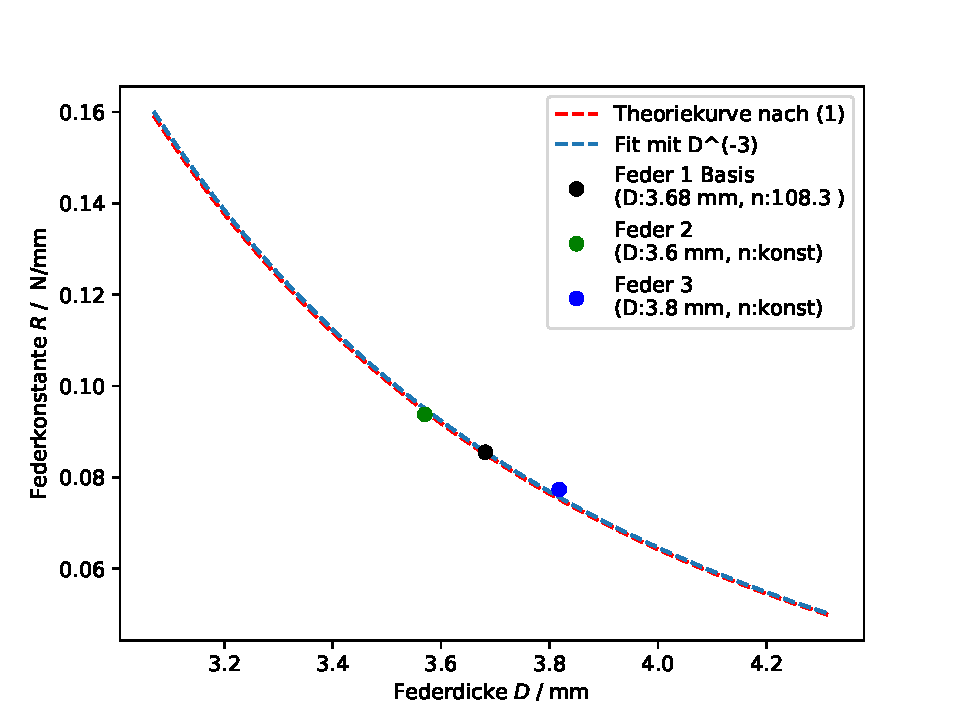
\includegraphics[width=\textwidth]{plots/opt_dicke_konstante_dia.pdf}
    \end{subfigure}
    \begin{subfigure}[c]{0.5\textwidth}
        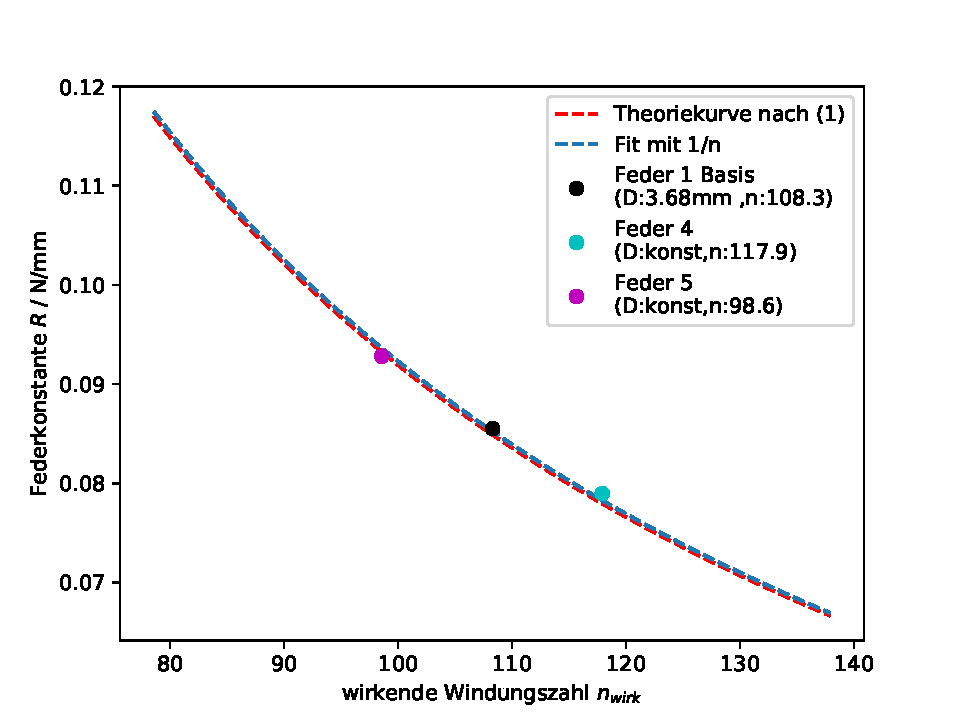
\includegraphics[width=\textwidth]{plots/opt_n_konstante_dia.pdf}
    \end{subfigure}
    \caption{Abb. \ref{fig:R_D_dia} (links) und \ref{fig:R_n_dia} (rechts) mit angenommener Drahtdicke $d_{ang}$}
\end{figure}

\newpage
\label{sec:aussagekraft}
\subsubsection{Einhaltung der Parameter der Basisfeder}
Nun sollen die Basisfeder mit der geforderten Feder aus der Federberechnung der
Firma Schnöring (Idealfeder) verglichen werden. Die Basisfeder ist dabei, die nach jenen
Berechnungen gefertigte Feder. Da es in der Praxis zu einigen Schwangungen in der
Fertigung kommen kann, soll nun überprüft werden, ob die zulässigen Schwankungen eingehalten werden.\\
Dazu wird die Federberechnung Anhang:\ref{fig:schn_b37} verwendet. 
\begin{figure}[H]
    \center
    \includegraphics[width=0.8\textwidth]{plots/schnö_12_dia.pdf}
    \caption{Dargestellt ist die geforderte Idealfeder nach Federberechnung der 
            Firma Schnöring im Vergleich mit der Basisfeder, welche nach diesen Berechnungen
            gefertigt wurde.
    }
    \label{fig:qual_basis}
\end{figure}

%Trotz der Differenz im Federaußendurchmesser $\Delta D_a=0.02\si{mm}$ und der Federlänge
%$\Delta L0=0.797\si{mm}$ gegenüber den aus der Federberechnung stammenden Werten, ist in
%Abb. \ref{fig:qual_basis} deutlich, dass die Basisfeder in dem vorgeschriebenen Kräftebereich
%für $F1$ und $F2$ liegt.
\begin{table}[H]
    \center
    \begin{tabular}{c |c c c c c}
        \toprule
        & $F0\;/\;N$ & $F1\;/\;N$ & $F2\;/\;N$ & $D_a\;/\;mm$ &$L0\;/\;mm$\\
        \midrule
        Basisfeder (Ist  )&0.73    &4.83   &8.0   &3.68  &57.06\\
        Idealfeder (Soll) &1.44    &5.00   &7.9   &3.70  &59.577 (58.0*)\\
        \midrule
        Abweichung $\;/\;$\% &49.3 &3.4    &1.25  &0.5   &4.2 (1.6) \\
        Abweichung        &0.71    &0.17   &0.1   &0.02  &2.517 (0.94)\\
        zul. Abweichung   &-       &0.25   &0.30  &0.1   &(2.0*)\\
        \bottomrule
    \end{tabular}
    \caption{Wertetabelle - Vergleich Basisfeder mit Idealfeder (Ist/Soll).\\
            *Stammt dabei aus der Federzeichnung \ref{fig:zeichnung}, da L0 ein
            anzustrebener Wert ist (vgl. dazu Abs. \ref{sec:praxis}).
    }
    \label{tab:vergleich}
\end{table}
\label{sec:einhaltung}

\subsection{Fazit}
Die in der Zeichnung \ref{fig:zeichnung} dargestellte Zugfeder (genauer: Trompentenfeder)
wurde in den Paramtern des Federausßendurchmessers $D_a$ und der Federgesamtlänge und somit auch
wirkenden Federwindungszahl $n_{wirk}$ variiert. Mit den Resultierden Kräften $F1$ und $F2$ an
$L1$ und $L2$ werden Aussagen über die innere Vorspannkraft $F0$ und der Federkonstante $R$ und derer
Abhängigkeiten zueinander gemacht. Dabei wird angenommen, dass der Ösenanteil (Trompetenanteil) 
im betrachteten Kräftebereich keine federnde Wirkung besitzt und somit eine Näherung einer
zylindrische Feder ohne Ösen verwendet wird.\\

Abschnitt \ref{sec:Auswertung} und \ref{sec:aussagekraft} zeigt, dass die gefertigten Federn 
bei Berücksichtigung der varrierende Drahtdicke $D_a$ der zu erwartenen 
Theorie aus Abschnitt \ref{sec:theorie} folgen.\\

Explizit zeigt dafür der Abschnitt \ref{sec:federdicke} und \ref{sec:federwindungen} die Proportionalitäten 
\begin{align*}
    R &\propto \frac{1}{n},\\
    R &\propto \frac{1}{D^3},\\
\end{align*}
auf.


Zudem liegen die Parameter von Feder 1 in den zulässigen Schwankungsbereichen 
der geforderten Feder resultierend aus der Federberechnung der Firma Schnöring (vgl. Abs. \ref{sec:einhaltung}).\\ 
Sodass diese als Ausgangsfeder (Basisfeder) verwendet werden kann.\\\\

Für die Materialzunahme...



%Im Folgenden können mit den gefertigten Federn weitere Aussagen getroffen werden,
%da sie der zu erwartenen Theorie aus Gl. \ref{eqn:federrate} folgen.   



%\begin{figure}
%    \center
%    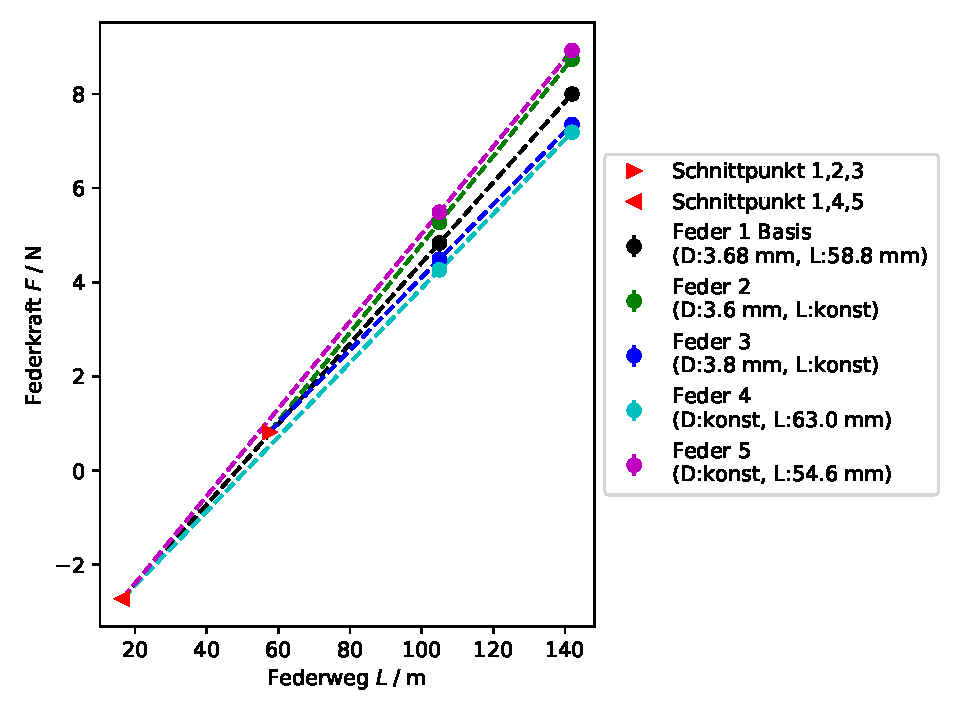
\includegraphics[width=0.8\textwidth]{plots/diss_kraft_dia.pdf}
%    \caption{
%        Vergleich der Wirkung der veränderlichen Windungszahl $n$ und
%        des Federaußendruchmesser $D_a$ auf die Federkraft $F$ untereinander.
%    }
%\end{figure}



